\section{Perceptron}

Das Perzeptron ist eine einfache Variante eines neuronalen Netzes. Das Prinzip wurde erstmals im Jahre 1958 von Frank Rosenblatt veröffentlicht\cite{rosenblatt58}. Es handelt sich dabei um eine lineare Diskriminantenfunktion. Während des Lernvorganges wird ein Vektor mit Gewichten erstellt, welcher dann anschließend eine Klassifikation vornimmt. Das Ergebnis wird anschließend durch eine Signum-Funktion dargestellt.

\subsection{Untersuchen sie den Trainingsalgorithmus: Welche Eigenschaften der Daten beeinflussen die durchschnittliche Anzahl an Iterationen bis eine Lösung w* gefunden wurde?}
Wenn die Daten linear separierbar sind kann immer eine obere Grenze für die Anzahl der Iterationen bis zur Konvergenz zu einer optimalen Lösung gefunden werden.
Die lineare Separierbarkeit ist eine Eigenschaft, welche die Anzahl der Schritte beeinflusst, je besser separierbar desto schnellere Konvergenz, weil die Verschiebung in jedem Schritt optimal ist. Allerdings ist bei nicht linear separierbaren Daten nicht garantiert, dass immer eine optimale Lösung gefunden wird. Außerdem terminiert der Algorithmus nie, weil die Daten ja nicht linear separiert werden können. \par{Es kommt auch darauf an, wie viele Elemente welcher Klasse existieren, wenn Klasse 1 viel mehr Elemente als Klasse 2 hat, wird die Entscheidungsgrenze so verschoben, dass Klasse 1 öfter richtig klassifiziert wird (weil ja mehr Elemente mehr zum Gewichtsvektor beitragen)}

\subsection{Welchen Einfluss hat die Schrittweite?}
Die Schrittweite oder Lernrate $\gamma$ kann man so verstehen, dass die Entscheidungsgrenze immer um den Richtungsvektor * Lernrate verschoben wird. Wenn die Lernrate zu groß wird, können optimale Lösungen übersprungen werden (wenn wir uns den Lösungsraum im Dreidimensionalen vorstellen, so kann ein Tal einfach übersprungen werden), ist die Lernrate zu klein, so kann es passieren, dass man in einem lokalen Optima stecken bleiben kann.

\subsection{Plotten Sie Daten und Entscheidungsgrenze (analog zu Punkt 1.1).}
\begin{figure}
	
	\centering
	\mbox{
		\subfigure[Nicely spread data]{
			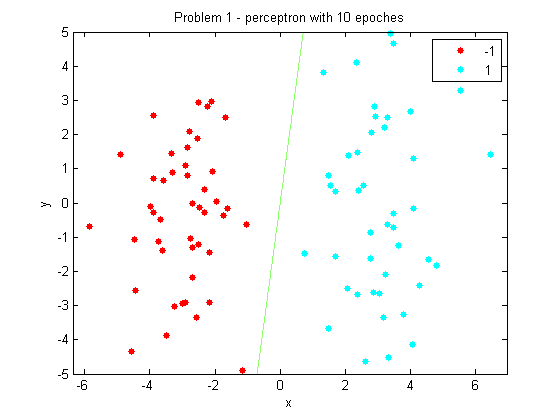
\includegraphics[width=60mm, trim = 0cm 0cm 0cm 0cm]{img/goodsep1.png}
		}
		
		\subfigure[seperable data but close together]{
			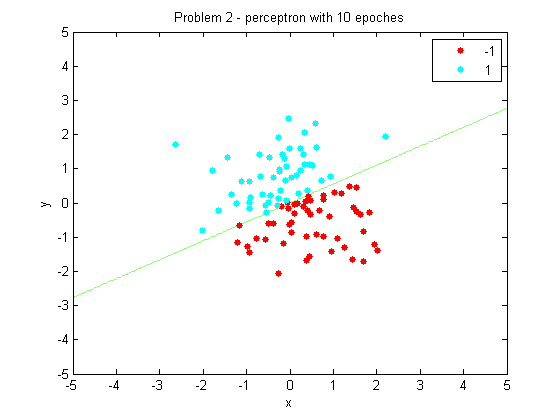
\includegraphics[width=60mm, trim = 0cm 0cm 0cm 0cm]{img/closesep2.png}
		}	
	}
	\mbox{
		\subfigure[Not seperable data]{
			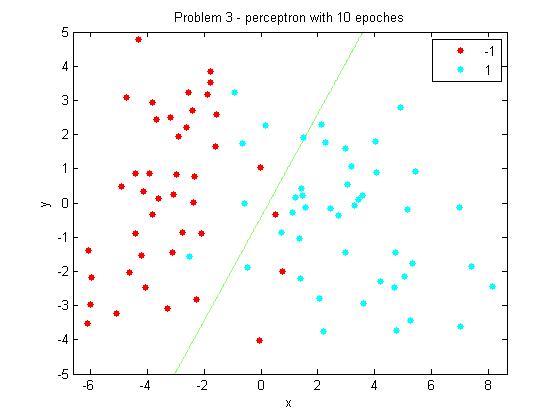
\includegraphics[width=60mm, trim = 0cm 0cm 0cm 0cm]{img/notsep3.png}
		}
	}
	
	\caption{Verschiedene Plots des Perceptron Klassifiers nach 10 Epochen}
	\label{fig:perceptron}
\end{figure}

\subsection{Vergleichen Sie das Perzeptron mit der Funktion memory. Worin liegt der Unterschied?}
Bei memory werden nur Punkte erkannt, die im Trainingsset vorhanden waren. Bei allen anderen Punkten ratet die memory Funktion. Das Perzeptron wiederum kann aufgrund der eingegangenen Daten generalisieren und damit Rückschlüsse auf neue Daten machen. Dadurch können neue, unbekannte Daten mit einer höheren Wahrscheinlichkeit richtig klassifiziert werden. Daher führt das Perzeptron eine Entscheidungsgrenze ein, welche dann für die neuen Daten angewandt werden kann. Dadurch wird das Overfitting vermindert oder ganz vermieden.


\subsection{Wie ist das Verhalten bei nicht linear separierbaren Daten?}
Die Entscheidungsgrenze bildet eine Ausgleichsgerade zwischen den zwei Klassen, wie in der Vorlesung gesehen, minimiert sie theoretisch den Abstand zu beiden Klassen, allerdings oszilliert sie in aufeinanderfolgenden Iterationen in der Region, in der sich die Klassen überlappen, weil jede falsche Klassifikation die Entscheidungsgrenze verschiebt, weil es aber immer falsche Klassifikationen geben wird, wird auch die Entscheidungsgrenze immer hin und her geschoben.